% !TeX root = ../main.tex

\chapter{后端}

\section{底层指令变换}

\subsection{ARM架构简介}

ARM是一个精简指令集(RISC)处理器架构家族统称,广泛应用在低功耗的嵌入式领域,同时在手机处理器市场上也占有绝对优势,最近的Apple M1 芯片也是ARM架构应用于电脑的成功尝试。

树莓派也是基于ARM架构的单片机电脑,基于Linux系统,在计算机和编程教育方面有着广泛的应用,根据树莓派基金会统计,截至2015年2月,已经售出超过500万台树莓派,这使得树莓派成为最畅销的英国“电脑”。同时,树莓派在简易服务器搭建,并行计算,机器人控制,甚至线上服务后端等各种领域都有着广泛的创意应用。

回到ARM架构上,Raspberry Pi 4 Model B是arm/EABI架构,有着一个1.5 GHz 64/32-bit 4核 ARM Cortex-A72处理器,这里比赛中要求采用32位模式。ARM Cortex-A72支持3路乱序超标量流水,有较多的通用寄存器,它们的作用如下


\begin{table}[htb]
  \centering\small
  \caption{ARM v8架构的寄存器作用说明}
  \label{tab:arm}
  \begin{tabular}{cl}
    \toprule
    ARM REG	 & Description	\\
    \midrule
    R0	& General Purpose	\\
    R1-R5 &	General Purpose \\
    R6-R10 &	General Purpose \\
    R11  &Frame Pointer \\
    R12	& Intra Procedural Call \\
    R13  &	Stack Pointer	\\
    R14  &	Link Register	\\
    R15  &	 Program Counter \\
    CPSR &	Current Program State Register/Flags    \\
    \bottomrule
  \end{tabular}
\end{table}

在IR级别的指令,与机器平台无关,因而可以设计实际机器并不支持的求余指令,减少变量数目,方便分析变换。而在翻译为汇编指令的时候,再用乘法除法和加法替代。经过寄存器分配后,可以使用通用寄存器和低频临时寄存器 r12 r14,进一步向底层翻译时,可用高频临时寄存器 r11,最终生成汇编码时,使用物理指,直接对应到 ARM 指令。


\subsection{底层指令转换}

\subsubsection{融合比较和分支指令}

在IR层级,编译器无法获得机器平台的信息,所以条件分支被设计成通用的先计算比较结果,再根据结果真假分支。了解到ARM v8支持根据比较结果直接分支时,在比较结果不会被其他地方用到时,编译器可以融合比较和分支指令:
融合前

$$
\text{i1 \%5  = CmpLT i32 \%4 i32 100 }
$$
$$
\text{Br i1 \%5 <label> \%6 <label> \%21}
$$
如果\%5不会在除了分支指令外的指令中用到,就可以进行这一变换

融合后:
$$
\text{Br LT i32 \%4 i32 100 <label> \%6 <label> \%21 }
$$

这样可以省掉虚拟变量\%5,并减少寄存器的使用。


\subsubsection{融合加法和乘法指令}

ARM架构的另一项指令集特征是;可以将移位和旋转操作融合为一条求地址的指令,此处移位操作是地址对齐因数,旋转操作表示从基址增加这个偏移量,举例来说,对于如下SysY指令:
$$
\text{a = a + (j  << 2);
}
$$

ARM架构可以用一条指令实现:
$$
\text{ADD  Ra, Ra, Rj, LSL \#2}
$$

这在取数组中变量的地址时很常用。


\section{寄存器分配}

\subsection{简介}

本项目的寄存器分配算法使用图染色算法实现,虽然图染色算法不是目前最优秀的的寄存器分配算法,而且也有复杂度较低且更易于实现的线性扫描算法,但是由于其经典性和不错的性能,所以本项目借鉴了线性扫描的思想,使用图染色的方法来进行寄存器分配。

算法的基本思想:

为了实现SSA中虚拟变量的define和use两个操作,需要保证某个变量在 use时其Value可以被访问到,即存储其Value的寄存器不应该被其他虚拟变量的Value覆盖,那么,我们有两种实现方式:

第一种,可以把虚拟变量的值存在栈上,即“不分配”,这种实现方式比较简单,优点是不需要考虑寄存器或CPU等目标机器平台特性,如JVM,便于移植,同时代码量较小,但是缺点是性能显然会由于频繁的读取存储器而较差。

第二种,把虚拟变量的值存在寄存器上,那么在这个变量的整个存活期被分配的寄存器都不应该被其他赋值覆盖。

\subsection{图染色算法}
寄存器分配算法的问题描述:

输入:一个有 N 个节点,k种可选颜色的无向图,节点代表某虚拟变量,颜色数代表可用的寄存器数

输出:所有变量的一个寄存器分配方案

图的k染色问题是一个NP难问题,算法的基本思想如下:

1. 如果max degree of nodes <    k那么总是能染色:把最大度数的节点删去,其他节点各分配一种颜色,至少会留下一种颜色给这个度数最大的节点

2. 如果max degree of nodes ≥ k 也是有可能 k 染色的:最简单的例子:星型图。我们只需把这些度数超过k的节点从图中删去(同时删去其邻边),判断新的图能否k-1染色

3. 如果删去所有度数大于k的节点后余下的图是一个完全图,且每个节点的度数大于k减去删除的节点数,那么这个图是不可以k染色的,我们需要选择抛出的节点,将其存入内存,通过Load操作访问,让其不参与寄存器分配


算法流程具体如下:

1. 把所有度数小于N的节点压栈(从图中暂时删除)同时删去邻边

2. 当图中所有节点度数大于N时,用启发式函数找到最应该被抛出的那个节点,删去此节点

3. 重复上述两个步骤直到图为空

4. 逐个弹出栈中元素,它们都是可染色的

5. 对于那些被删除的节点(暂时spill)两种解决方案: Chaitin 的算法认为这种节点只能抛出,Briggs 改进算法认为可以通过 split 分裂一个live range 为多个来实现重新染色\cite{10.1145/177492.177575} ,这里本项目采用简单的抛出。





\subsection{算法实现和案例}


1. 对于基本块的OUT集合中的虚拟变量,它们的存活期是整个基本块,所以它们的remains初始化为1,也即整个基本块中它们存在的寄存器都处于占用状态

2. 自前向后的对于每条指令,余下的基本块部分如果该指令用到了某个虚拟变量,就可以把它的remains减一,模拟线性扫描算法中某个变量存活期所跨越的指令数,当remains减至0时,就说明后边儿不会再使用此变量了,该寄存器得以释放

我们需要两个数据结构:用于记录变量冲突图的Interface Graph和模拟变量存活期的remians,下面将结合图~\ref{fig:regAlloc}来说明这remains数据结构的作用:

\begin{figure}[htb]
  \centering
  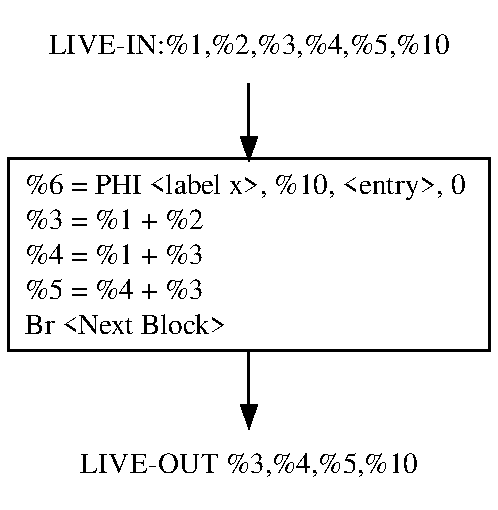
\includegraphics[width=0.4\textwidth]{figures/reg_alloc.pdf}
  \caption{在块内执行寄存器分配的示例}
  \label{fig:regAlloc}
  \note{注:LIVE-IN表示经过数据流分析后,在该基本块需要的变量,LIVE-OUT表示数据流分析中,在该基本块之后仍然被需要的变量。}
\end{figure}


本项目中寄存器分配在基本块级别进行,所以第一步是进行数据流分析,得到从前驱进入该基本块的变量和被该基本块后继需要的变量。对于活跃进入该基本块的变量,本项目中假定它们在之前的基本块内寄存器分配时被分配了寄存器,在出口处不活跃的变量,只需活跃到最后一次使用它的指令的地方即可,否则,应该在基本块结束时确保它们已经被分配到寄存器中。按照上述规定,该案例的所有变量的活跃期如图~\ref{fig:regAllocLiveRange}

\begin{figure}[htb]
  \centering
  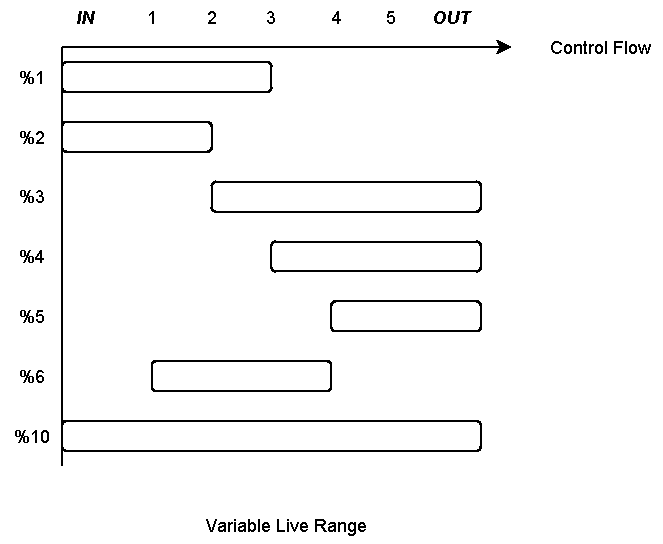
\includegraphics[width=0.8\textwidth]{figures/reg_live_range.pdf}
  \caption{图~\ref{fig:regAlloc}中的虚拟变量关于指令次序的存活期}
  \label{fig:regAllocLiveRange}
\end{figure}

对于变量\%1和\%2,由于\%1在出口处不活跃,所以只需要从活跃到最后一条使用\%1的指令,即第三条指令处;变量\%2 与之类似;变量\%3,\%4和\%5,这些变量都在出口处活跃,所以他们的活跃期应该是自赋值指令起,到基本块的;变量\%6属于基本块内定义的变量,而且不在出口处活跃,所以只需要从定义处活跃到最后一次使用\%6的指令,即第四条指令处;变量\%10同时在入口处和出口处活跃,因而在寄存器充分的情况下可以将其一直保留在寄存器中,否则,至少需要一对存取操作。

由此,自上而下的分析每条指令,该指令的左值应该与此时所有活跃的变量冲突,构建得到冲突图,如图~\ref{fig:graph0}。

\begin{figure}[htb]
  \centering
  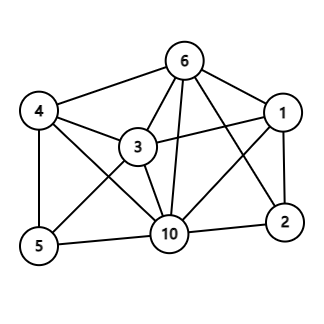
\includegraphics[width=0.3\textwidth]{figures/graph.png}
  \caption{冲突图}
  \label{fig:graph0}
\end{figure}
按照算法,逐个把度数最小的节点入栈,这些度数小于k的节点一定可以染色。节点5的度数为3,将其入栈,得到图~\ref{fig:graph1}。

\begin{figure}[htb]
  \centering
  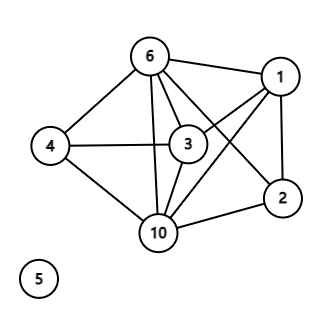
\includegraphics[width=0.3\textwidth]{figures/graph1.png}
  \caption{删去节点5}
  \label{fig:graph1}
\end{figure}

当删去5的邻边后,节点4成为度数最小的节点之一,删去节点4,此时的冲突图如图~\ref{fig:graph2}:

\begin{figure}[htb]
  \centering
  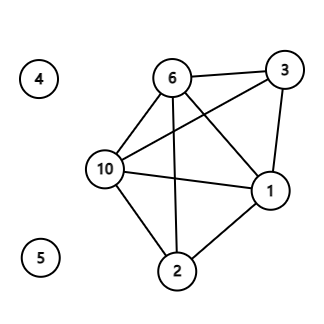
\includegraphics[width=0.3\textwidth]{figures/graph2.png}
  \caption{删去节点4}
  \label{fig:graph2}
\end{figure}

同理,删去节点3得到图~\ref{fig:graph3},此时的冲突图是一个4-完全图。

\begin{figure}[htb]
  \centering
  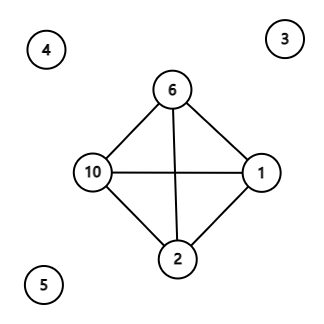
\includegraphics[width=0.3\textwidth]{figures/graph3.png}
  \caption{删去节点3}
  \label{fig:graph3}
\end{figure}

因为我们有4个可用寄存器,因此这些节点都可以被染色,不妨按照红黄蓝绿的次序给节点1,2,6,10分别染色,依次弹出栈中元素3,4,5。对之前弹出的节点进行染色,节点3与节点6,10冲突,因此可选颜色为红色或黄色,不妨假定为红色;节点4与3,6,10冲突,只能为黄色;节点5与3,4,10冲突,只能为蓝色,至此一种4染色的方案就完成了。
